\documentclass[12pt,a4paper]{article}
\pagestyle{plain}
\usepackage{fullpage}
\usepackage[english]{babel}
\usepackage{enumerate}

%equations
\usepackage[fleqn]{amsmath}
\numberwithin{equation}{section}

%figures
\usepackage[dvips]{graphicx}
\graphicspath{{./images/}}
\numberwithin{figure}{section}

%excercises
\newcounter{Exercise}
\setcounter{Exercise}{1}
\usepackage[dvipsnames]{xcolor}
\usepackage{framed}
\definecolor{shadecolor}{gray}{0.9}
\usepackage{caption}

%tables
\numberwithin{table}{section}

%specials
\usepackage{textcomp} %special (greek) characters as text
%\usepackage{pstricks} %
%\usepackage{ifthen} %
%\usepackage{calc} %
\usepackage{isotope}
\usepackage{hyperref}
\usepackage[bottom]{footmisc} %footnote below figure
\usepackage{footnpag}%number footnotes per page


%document details
\author{N.G. Schultheiss \\ translated and adapted by K. Schadenberg}
\date{}
\title{Standard Model - Forces}


\begin{document}
\maketitle

\section{Introduction}
In the previous module `Standard Model - Particles' we already showed a large a part of the standard model, the particles. In this module we look at the other large part of the model, forces. The forces have their own particles, carriers, associated with them. In this text we will use the decay of a neutron as an example to show the possible interactions with and between force particles.

\section{Forces}
A force we cannot ignore as human here on Earth is gravity. It keeps our feet firm on the ground. The behaviour of gravity can be described using the following equation:
\begin{equation}
F_{\mbox{gravity}} = G \frac{m_1 m_2}{r^2}
\end{equation}

The second very familiar force is the electrical force. Electrons are bound to the positively charged nucleus of an atom by this force. The description of the behaviour of the electrical force:
\begin{equation}
F_{\mbox{electric}} = \frac{1}{4 \pi \epsilon_0} \frac{q_1 q_2}{r^2}
\end{equation}
This electrical force is much stronger than gravity. It takes the entire mass of the Earth to keep us on the ground but a chair, which is held together by electrical forces, is strong enough to overcome this force.

\begin{shaded}
\textbf{Exercise \theExercise \stepcounter{Exercise}} : Compare the gravitational constant $G$ with the vacuum permittivity (also called electric constant) $\epsilon_0$. What does this mean for the gravitational and electrical forces?\end{shaded}

There are two more forces in the standard model which are perhaps a little less familiar; the strong and weak (nuclear) force. Weak interaction is the driving force behind nuclear decay and flavour changes in quarks. The strong force, as indicated by its name, is stronger and holds protons and neutron together inside the nucleus of atoms. But it also holds together the quarks which make up these hadrons. Where other forces decrease in strength with increasing distance, the strong force actually becomes stronger.

\section{Neutron Decay}
Neutrons are not stable particles, outside the nucleus they decay in a matter of minutes according to the following reaction:
\begin{equation}
\isotope[1][0]{n} = \isotope[1][1]{p} + \isotope[0][-1]{e} + \isotope[0][0]{\bar{\nu}} \label{eq:neut_decay}
\end{equation}

This reaction shows a lot of the rules (laws) all reactions much abide by:
\begin{itemize}
\item The number of hadrons (baryons in this case) is constant.
\item The number of other particles (leptops) is constant. Although there are more particles on the right hand side of the equation, one of the new particles is an anti particle negating the creation of the second new particle.
\item The charge is the same on both sides of the equation. A single neutron has no charge and the charges of the proton and electron combined also gives a neutral charge.
\end{itemize}

A different way of describing the reaction above is by using a diagram or drawing. A standard way of representing particle interactions is using Feynman-diagrams. The diagram for neutron decay is shown in figure~\ref{fig:Feyn_Neutron}. In this diagram the first of our new force-particles takes centre stage. The conversion of a neutron into a proton is governed by the W$^-$-boson. A neutron consists of two down quarks and one up quark; udd. A proton on the other hand has the quark combination uud. We can therefore say that a single d-quark changes into an u-quark while emitting a W$^-$-boson. This W$^-$-boson then decays into an electron and an anti-neutrino.

\begin{figure}\begin{center}
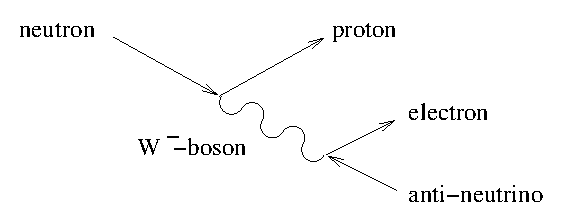
\includegraphics[scale=1]{Feyn_Neutron.eps}%
\caption{A first-order Feynman-diagram showing neutron decay.}\label{fig:Feyn_Neutron}
\end{center}\end{figure}

The convention for Feynman diagrams is that time runs from left to right. This means that in figure~\ref{fig:Feyn_Neutron} the neutron, proton, and electron follow the arrow of time, they travel with time. The anti-neutrino on the other hand travels against time. It can also be seen as a particle which disappears from nothingness, leaving behind an anti-particle.

The Feynman-diagram works both ways, we can very easily reverse the arrow of time. Now we have an neutrino colliding with an anti-electron. By changing time our charges also change (particles change into anti-particles and vice-versa). The W$^-$-boson now becomes a W$^+$-boson which collides with an anti-proton creating an anti-neutron.

But we can also let the time run in other directions, from top to bottom for instance. The reaction then becomes a neutron colliding with an anti-proton creating a W$^+$-boson. The boson decays into a neutrino and an anti-electron. At first glance this might seem a perfectly valid reaction. However, in the module `Standard Model - Particles' we described how we can write neutrons and protons as combinations of quarks. A neutron is udd, a protons is uud, and our new anti-proton is $\overline{\mbox{uud}}$. We now have three quarks changing into three different quarks while there is only one boson present, not possible. If we redraw our Feynman-diagram using the symbols u and d for the quarks, and the changes that occur we obtain a valid figure in which we can point the arrow of time in any direction, see figure~\ref{fig:Feyn_Neutron2}.

\begin{figure}\begin{center}
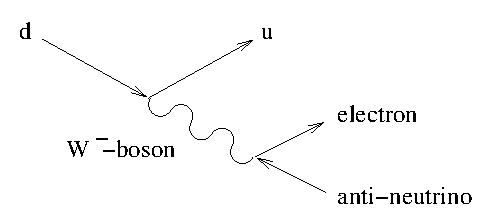
\includegraphics[scale=1]{Feyn_Neutron2.eps}%
\caption{The correct version of the Feynman-diagram shown in figure~\ref{fig:Feyn_Neutron}.}\label{fig:Feyn_Neutron2}
\end{center}\end{figure}

A third boson connected to the weak interaction which we have not mentioned in the previous example of a decaying neutron is the neutral Z-boson. In every reaction we have to make sure that the charge before and after are the same. A negatively charged W$^-$-boson can for instance decay into an electron and an anti-neutrino or a quark and anti-quark of the right charge. Recall from the previous module that quarks have fractional electrical charges: $\pm~1/3~e$ or $\pm~2/3~e$. With the decay of an W$^-$-boson one -1/3e quark and one -2/3e quark must form. Of course instead of a electron it is also possible to create a muon or tauon. With the decay of a W$^+$-boson positive leptons must be created of a pair of positive quarks.

Because the Z-boson has no charge, the sum of the charges of the decay products must also be neutral. This can either be a lepton with its anti-lepton (with opposite charges or both no charge) or a quark anti-quark pair.

\section{Forces inside the Nucleus}
In the previous section we saw that the decay of a neutron into a proton involves the emission of a W$^-$-boson. This W$^-$-boson can be seen as the carrier of the weak (nuclear) force. We can rewrite the reaction of \ref{eq:neut_decay} into a reaction between quarks. Take a look at figure~\ref{fig:neut_dacay_quark}.

\begin{figure}\begin{center}
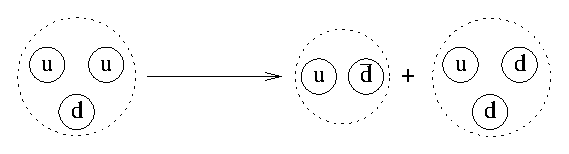
\includegraphics[scale=1]{neut_dacay_quark.eps}%
\caption{Neutron decay on the quark level.}\label{fig:neut_dacay_quark}
\end{center}\end{figure}

In this figure a pair of quarks, u$\bar{\mbox{d}}$, takes the place of the W$^-$-boson. The u$\bar{\mbox{d}}$-particle is called the $\pi^-$ or negative pion. At first it was thought that this pion was responsible for the decay of neutrons and the weak force as a whole.

The pion is part of a new group of particles, the mesons. Mesons are composed of a pair of quarks, one of which is a `normal' quark the other is an anti-quark. Mesons therefore are a part of the larger boson family.

One of the problems physicists struggled with before the discovery of the W$^-$-boson and pions was the stability of atomic nuclei. A nucleus only contains positive and neutral charges. What prevents the protons from flying away, out of the nucleus? With the discovery of the pion physicists thought they had found the glue that hold the nucleus together. Hideki Yukawa (1907-1981) reasoning was as follows:
\begin{itemize}
\item The electrical force is quantised by photons. Each individual photon carries a part of the electrical force.
\item Photons have an integer spin number, this means that they are, together with pions, part of the boson family.
\item In a Bose-Einstein condensate, a group of particles forms a single quantum mechanical unit. Perhaps bosons have the property of `merging things'.
\item The force between protons and neutrons might be carried by bosons. Perhaps all forces are carried by bosons.
\item According to the Heisenberg uncertainty principle ($\Delta E \Delta t > \hbar$) we can either measure the energy or time with a high accuracy, but not both at the same time.
\item This allows us to `borrow' some energy for a short period of time as long as $\Delta E \Delta t < \hbar$, because this lending of energy cannot be measured.
\item Using $E=mc^2$ we can convert this energy into a particle, but this particle can only exist for a short time. This particle might resemble the pion.
\end{itemize}

Figure~\ref{fig:borrowing_energy} shows how this works with our neutron and proton. We borrow some energy from the proton to create a short lived particle. This particle has to disappear very fast and can therefore not travel very far before it is absorbed by a different nucleon (figure~\ref{fig:neut_dacay_quark}). Following this reasoning the particle acts like a force.

\begin{figure}\begin{center}
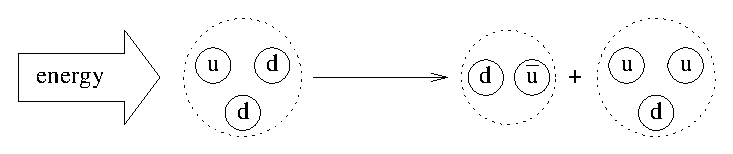
\includegraphics[scale=1]{borrowing_energy.eps}%
\caption{Borrowing energy from a proton.}\label{fig:borrowing_energy}
\end{center}\end{figure}

There are three types of pions: $\pi^+$, $\pi^0$, and $\pi^-$. They consists of up, down, anti-up, and anti-down quarks. To create the neutral $\pi^0$ you need to combine an up with an anti-up or a down with an anti-down quark.

\begin{shaded}
\textbf{Exercise \theExercise \stepcounter{Exercise}} : Which combinations of quarks are needed to create the $\pi^+$ and $\pi^-$ particles?\footnotemark\end{shaded}
\footnotetext{The properties of the different quarks can be found in the module `Standard Model - Particles'.}
\begin{shaded}
\textbf{Exercise \theExercise \stepcounter{Exercise}} : Calculate the lifetime of a pion given $\hbar=1.0545 \cdot 10^{-34}$~Js, the mass of $\pi^0$ is roughly $135 \frac{\mbox{MeV}}{c^2}$, and the mass of $\pi^+$ and  $\pi^-$ equals $140 \frac{\mbox{MeV}}{c^2}$.

How much energy must be borrowed to create the pion? How long can we borrow this energy without violating Heisenberg's uncertainty principle?\end{shaded}
\begin{shaded}
\textbf{Exercise \theExercise \stepcounter{Exercise}} : How far can a pion travel during its lifetime if it moves at the speed of light?\end{shaded}

According to the internet\footnote{And the internet knows everything and is never wrong.}~the composition of a $\pi^0$ particle is $\frac{\mbox{u}\bar{\mbox{u}}+\mbox{d}\bar{\mbox{d}}}{\sqrt{2}}$. Apparently a $\pi^0$ is a mix of two different possible combinations of quarks. These two possibilities are perpendicular to each other. Dividing by $\sqrt{2}$, the length of these possibilities laid end to end, gives us one average particle.

\begin{figure}\begin{center}
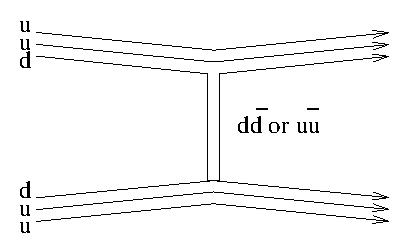
\includegraphics[scale=1]{meson_exchange.eps}%
\caption{The force between two baryons shown as the exchange of a meson.}\label{fig:meson_exchange}
\end{center}\end{figure}

\section{The Strong Force}
Hadrons contain charged quarks and/or anti-quarks. How do these charged particles stay together? The two up quarks inside a proton repel each other much stronger than the down quark can keep them together.

A second problem is that quarks are fermions. This means that two quarks cannot occupy the same quantum state. To describe a proton or neutron we need a new quantum property. Because there are three quarks / anti-quarks in a baryon and a quark anti-quark pair in a meson there are six possible states for every quark. We have given these states colours: red, green, blue, anti-red, anti-green, and anti-blue.

Combining red, green, and blue light gives us white light. In a similar fashion quark colours combine to make new colours. Anti-red combined with red will also result into white. This allows us to make a large number of different possibilities. But only white is allowed as end result. The strong (nuclear) force will make sure of this.

The strong force constantly exchanges the colours between quarks. The carriers of the strong force are called gluons, glue particles keeping everything together. A red quark can emit a red gluon. But this red quark can also change colour to become green. However, the mix of colours must remain white. When the quark changes colour from red to green it emits a red / anti-green gluon. This gluon can interact with other gluons, or change the colour of a green quark into red.

Gluons are bosons, this means they do not need to obey the Pauli exclusion principle. Gluons can be stacked on top of each other and occupy the same quantum state. Also, the `direction' of gluons is unknown. The interaction caused by a r$\bar{\mbox{g}}$-gluon could just as well be the result of a $\bar{\mbox{r}}$g going the opposite way. We can write this particle as$\frac{\bar{\mbox{rg}}+\mbox{r}\bar{\mbox{g}}}{\sqrt{2}}$. This is one possible gluon colour combination. Figure~\ref{fig:gluon1} shows how these gluons keeps baryons and mesons together and how they cause the colour changes of the quarks inside.

With three colours (red, green, and blue) and two states (e.g. red and anti-red) we obtain eight ($2^3$) possible combinations. Five of these combinations are real and two are imaginary (complex).\footnote{This is only a very brief introduction into the colours of gluons and the rules associated with them. Sorting out the entire theory might be a good research assignment. Look for terms like quantum chromo dynamics and SU(3).} Although there are theories about hadrons containing only gluons, `glueballs'.

Baryons can decay into lighter baryons while emitting a meson. It is also possible for a baryon to emit a W$^-$-, W$^+$-, W$^0$-, or Z-boson and decay. The emission of a meson is shown in figure~\ref{fig:gluon2}

\begin{figure}\begin{center}
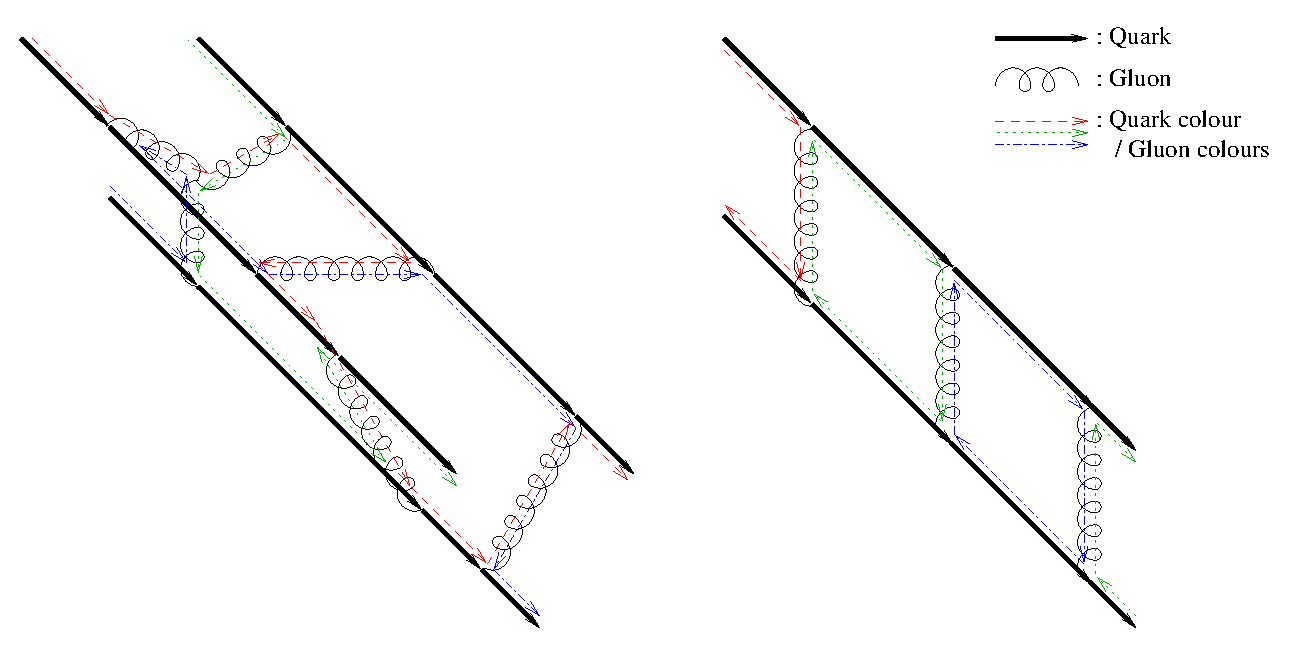
\includegraphics[scale=0.7]{gluon1.eps}%
\caption{Gluons keeping baryons and mesons together.}\label{fig:gluon1}
\end{center}\end{figure}

\begin{figure}\begin{center}
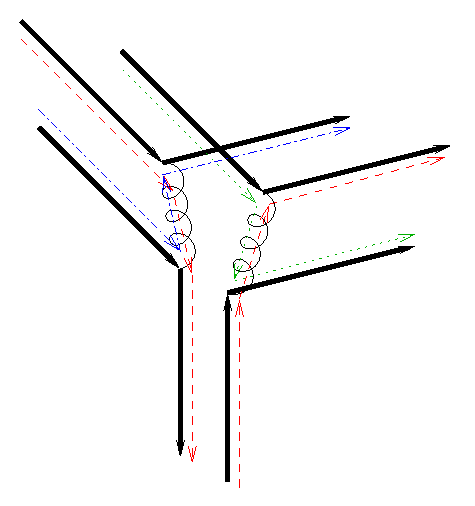
\includegraphics[scale=1]{gluon2.eps}%
\caption{Interactions by gluons between baryons and mesons.}\label{fig:gluon2}
\end{center}\end{figure}

\end{document}

